\documentclass[
11pt, % Main document font size
a4paper, % Paper type, use 'letterpaper' for US Letter paper
oneside, % One page layout (no page indentation)
%twoside, % Two page layout (page indentation for binding and different headers)
headinclude,footinclude, % Extra spacing for the header and footer
BCOR5mm, % Binding correction
]{book}

%%%%%%%%%%%%%%%%%%%%%%%%%%%%%%%%%%%%%%%%%
% Arsclassica Article
% Structure Specification File
%
% This file has been downloaded from:
% http://www.LaTeXTemplates.com
%
% Original author:
% Lorenzo Pantieri (http://www.lorenzopantieri.net) with extensive modifications by:
% Vel (vel@latextemplates.com)
%
% License:
% CC BY-NC-SA 3.0 (http://creativecommons.org/licenses/by-nc-sa/3.0/)
%
%%%%%%%%%%%%%%%%%%%%%%%%%%%%%%%%%%%%%%%%%

%----------------------------------------------------------------------------------------
%	REQUIRED PACKAGES
%----------------------------------------------------------------------------------------

\usepackage[
% nochapters, % Turn off chapters since this is an article        
beramono, % Use the Bera Mono font for monospaced text (\texttt)
eulermath,% Use the Euler font for mathematics
pdfspacing, % Makes use of pdftex’ letter spacing capabilities via the microtype package
dottedtoc % Dotted lines leading to the page numbers in the table of contents
]{classicthesis} % The layout is based on the Classic Thesis style

\usepackage{arsclassica} % Modifies the Classic Thesis package

\usepackage[T1]{fontenc} % Use 8-bit encoding that has 256 glyphs

\usepackage[utf8]{inputenc} % Required for including letters with accents

\usepackage{graphicx} % Required for including images
\graphicspath{{Figures/}} % Set the default folder for images

\usepackage{enumitem} % Required for manipulating the whitespace between and within lists

\usepackage{lipsum} % Used for inserting dummy 'Lorem ipsum' text into the template

\usepackage{subfig} % Required for creating figures with multiple parts (subfigures)

\usepackage{amsmath,amssymb,amsthm} % For including math equations, theorems, symbols, etc

\usepackage{varioref} % More descriptive referencing

\usepackage{tikz}
\setlength{\parskip}{0em}
\usetikzlibrary{decorations.pathmorphing,patterns}
\usepackage[american,cuteinductors]{circuitikz}
\usetikzlibrary{shapes,arrows,circuits,calc,babel}
% Definition of blocks:
\tikzset{%
  block/.style    = {draw, thick, rectangle, minimum height = 3em,
    minimum width = 3em},
  sum/.style      = {draw, circle, node distance = 2cm}, % Adder
  input/.style    = {coordinate}, % Input
  output/.style   = {coordinate} % Output
}
% Defining string as labels of certain blocks.
\newcommand{\suma}{\Large$+$}
\newcommand{\inte}{$\displaystyle \int$}
\newcommand{\derv}{\huge$\frac{d}{dt}$}


%----------------------------------------------------------------------------------------
%	THEOREM STYLES
%---------------------------------------------------------------------------------------

\theoremstyle{definition} % Define theorem styles here based on the definition style (used for definitions and examples)
\newtheorem{definition}{Definition}

\theoremstyle{plain} % Define theorem styles here based on the plain style (used for theorems, lemmas, propositions)
\newtheorem{theorem}{Theorem}

\theoremstyle{remark} % Define theorem styles here based on the remark style (used for remarks and notes)

%----------------------------------------------------------------------------------------
%	HYPERLINKS
%---------------------------------------------------------------------------------------

\hypersetup{
%draft, % Uncomment to remove all links (useful for printing in black and white)
colorlinks=true, breaklinks=true, bookmarks=true,bookmarksnumbered,
urlcolor=webbrown, linkcolor=RoyalBlue, citecolor=webgreen, % Link colors
pdftitle={}, % PDF title
pdfauthor={\textcopyright}, % PDF Author
pdfsubject={}, % PDF Subject
pdfkeywords={}, % PDF Keywords
pdfcreator={pdfLaTeX}, % PDF Creator
pdfproducer={LaTeX with hyperref and ClassicThesis} % PDF producer
}


%-------------------------------------------------------------------------------
% Custom math commands
%-------------------------------------------------------------------------------
\def\mf{\ensuremath\mathbf}
\def\mb{\ensuremath\mathbb}
\def\mc{\ensuremath\mathcal}
\def\lp{\ensuremath\left(}
\def\rp{\ensuremath\right)}
\def\lv{\ensuremath\left\lvert}
\def\rv{\ensuremath\right\rvert}
\def\lV{\ensuremath\left\lVert}
\def\rV{\ensuremath\right\rVert}
\def\lc{\ensuremath\left\{}
\def\rc{\ensuremath\right\}}
\def\ls{\ensuremath\left[}
\def\rs{\ensuremath\right]}
\def\bmx{\ensuremath\begin{bmatrix}}
\def\emx{\ensuremath\end{bmatrix}}
\def\bmx{\ensuremath\begin{bmatrix*}[r]}
\def\emx{\ensuremath\end{bmatrix*}}
\def\bmxc{\ensuremath\begin{bmatrix*}[c]}
    
% \def\bmxc{\ensuremath\begin{bmatrix}}

\newcommand{\demoex}[2]{\onslide<#1->\begin{color}{black!60} #2 \end{color}}
\newcommand{\demoexc}[3]{\onslide<#1->\begin{color}{#2} #3 \end{color}}
\newcommand{\anim}[3]{\onslide<#1->{\begin{color}{#2!60} #3 \end{color}}}
\newcommand{\ct}[1]{\lp #1\rp}
\newcommand{\dt}[1]{\ls #1\rs}
\newcommand{\cols}[2]{\begin{columns}[#1] #2 \end{columns}}
\newcommand{\col}[2]{\begin{column}{#1} #2 \end{column}}
\newcommand{\eqnwl}[1]{\begin{equation} #1 \end{equation}}
\newcommand{\eqnwol}[1]{\begin{equation*} #1 \end{equation*}}

\newcommand{\pp}[1]{\lp #1\rp}
\newcommand{\bb}[1]{\left[ #1\right]}
\newcommand{\cc}[1]{\left\{ #1\right\}}

 % Include the structure.tex file which specified the document structure and layout

\hyphenation{Fortran hy-phen-ation} % Specify custom hyphenation points in words with dashes where you would like hyphenation to occur, or alternatively, don't put any dashes in a word to stop hyphenation altogether

\usepackage{amssymb}
\usepackage{mathtools}
\usepackage{xcolor}


\def\mf{\ensuremath\mathbf}
\def\mb{\ensuremath\mathbb}
\def\lp{\ensuremath\left(}
\def\rp{\ensuremath\right)}
\def\lv{\ensuremath\left\lvert}
\def\rv{\ensuremath\right\rvert}
\def\lV{\ensuremath\left\lVert}
\def\rV{\ensuremath\right\rVert}
\def\lc{\ensuremath\left\{}
\def\rc{\ensuremath\right\}}
\def\ls{\ensuremath\left[}
\def\rs{\ensuremath\right]}
\def\bmx{\ensuremath\begin{bmatrix*}[r]}
\def\emx{\ensuremath\end{bmatrix*}}
\def\bmxc{\ensuremath\begin{bmatrix*}[c]}
 

\newcommand{\thrm}[2]{{\color{blue}#1}\vspace{0.25cm} \\ {\setlength{\parindent}{0cm} \textbf{Proof: } #2 $\blacksquare$}}


%----------------------------------------------------------------------------------------
%	TITLE AND AUTHOR(S)
%----------------------------------------------------------------------------------------

\title{
    \LARGE{Applied Linear Algebra in Data Analysis} \\
    {\color{gray} Tutorial}
} % The article title

% \subtitle{{Tutorial}} % Uncomment to display a subtitle

\author{{Sivakumar Balasubramanian}} % The article author(s) - author affiliations need to be specified in the AUTHOR AFFILIATIONS block

\date{} % An optional date to appear under the author(s)

%----------------------------------------------------------------------------------------

\begin{document}

%----------------------------------------------------------------------------------------
%	HEADERS
%----------------------------------------------------------------------------------------

\renewcommand{\sectionmark}[1]{\markright{\spacedlowsmallcaps{#1}}} % The header for all pages (oneside) or for even pages (twoside)
%\renewcommand{\subsectionmark}[1]{\markright{\thesubsection~#1}} % Uncomment when using the twoside option - this modifies the header on odd pages
\lehead{\mbox{\llap{\small\thepage\kern1em\color{halfgray} \vline}\color{halfgray}\hspace{0.5em}\rightmark\hfil}} % The header style

\pagestyle{scrheadings} % Enable the headers specified in this block

%----------------------------------------------------------------------------------------
%	TABLE OF CONTENTS & LISTS OF FIGURES AND TABLES
%----------------------------------------------------------------------------------------

\maketitle % Print the title/author/date block

\setcounter{tocdepth}{2} % Set the depth of the table of contents to show sections and subsections only

\tableofcontents % Print the table of contents

%\listoffigures % Print the list of figures

%\listoftables % Print the list of tables

\newpage % Start the article content on the second page, remove this if you have a longer abstract that goes onto the second page

\documentclass[12pt]{article}

\usepackage[utf8]{inputenc}
\usepackage{geometry}
\geometry{
    a4paper,
    total={170mm,257mm},
    left=25mm,
    right=25mm,
    top=25mm,
    bottom=25mm,
}
\usepackage{multicol}
\usepackage[font=small,labelfont=bf]{caption}
\setlength{\columnsep}{0.25cm}
\usepackage[inline]{enumitem}
\usepackage{amssymb}
\usepackage{xcolor}
\usepackage{mathtools} 
\setlength{\parindent}{0em}
\setlength{\parsep}{0em}
\usepackage{tikz}
\setlength{\parskip}{0em}
\usetikzlibrary{decorations.pathmorphing,patterns}
\usepackage[american,cuteinductors]{circuitikz}
\usetikzlibrary{shapes,arrows,circuits,calc,babel}
% Definition of blocks:
\tikzset{%
  block/.style    = {draw, thick, rectangle, minimum height = 3em,
    minimum width = 3em},
  sum/.style      = {draw, circle, node distance = 2cm}, % Adder
  input/.style    = {coordinate}, % Input
  output/.style   = {coordinate} % Output
}
% Defining string as labels of certain blocks.
\newcommand{\suma}{\Large$+$}
\newcommand{\inte}{$\displaystyle \int$}
\newcommand{\derv}{\huge$\frac{d}{dt}$}

\def\mf{\ensuremath\mathbf}
\def\mb{\ensuremath\mathbb}
\def\mc{\ensuremath\mathcal}
\def\lp{\ensuremath\left(}
\def\rp{\ensuremath\right)}
\def\lv{\ensuremath\left\lvert}
\def\rv{\ensuremath\right\rvert}
\def\lV{\ensuremath\left\lVert}
\def\rV{\ensuremath\right\rVert}
\def\lc{\ensuremath\left\{}
\def\rc{\ensuremath\right\}}
\def\ls{\ensuremath\left[}
\def\rs{\ensuremath\right]}
\def\bmx{\ensuremath\begin{bmatrix*}[r]}
\def\emx{\ensuremath\end{bmatrix*}}
\def\bmxc{\ensuremath\begin{bmatrix*}[c]}
\def\emxc{\ensuremath\end{bmatrix*}}
% \def\t{\lp t\rp}
% \def\k{\ls k\rs}

\newcommand{\demoex}[2]{\onslide<#1->\begin{color}{black!60} #2 \end{color}}
\newcommand{\demoexc}[3]{\onslide<#1->\begin{color}{#2} #3 \end{color}}
\newcommand{\anim}[3]{\onslide<#1->{\begin{color}{#2!60} #3 \end{color}}}
\newcommand{\ct}[1]{\lp #1\rp}
\newcommand{\dt}[1]{\ls #1\rs}

% \renewcommand{\familydefault}{\sfdefault}

\begin{document}
\begin{center}
\begin{large}
\textbf{Applied Linear Algebra in Data Analaysis}\\
\vspace{0.1cm}
\end{large}
\textbf{Vectors Assignment}
\end{center}
\hrule
\vspace{1em}

\begin{large}
    \textbf{Marks: 32}
\end{large}

\begin{enumerate}
    \item Is this set of vectors $\left\{\begin{bmatrix}2 \\ 1 \\ 1\end{bmatrix}, \begin{bmatrix}0 \\ 0\\ 0\end{bmatrix}, \begin{bmatrix}0 \\ 1 \\ 0\end{bmatrix}\right\}$ independent? 
    
    Explain your answer. \textbf{[Marks: 2]}

    \item Consider a set of finite duration discrete-time real signals \textbf{[Marks: 2]}
    \[ X_N = \lc x\dt{n} \big\vert x\dt{n} \in \mb{R}, \,\forall 0 \leq n \leq N-1\rc \]
    
    Does this set form a vector space? Explain your answer. Would $X_N$ still be a vector spaces if the signals were binary signals? i.e. $x\dt{n} \in \mb{B}$, where $\mb{B} = \lc 0, 1\rc$ with the binary addition and multiplication operations defined as the following,

    \begin{center}
        \begin{minipage}[h]{.45\textwidth}
            \centering
            \begin{tabular}{|c|c|c|c|}
                \hline
                $a$ & $b$ & $a+b$ & $a \times b$ \\ \hline
                0 & 0 & 0   & 0     \\ \hline
                0 & 1 & 1   & 0     \\ \hline
                1 & 0 & 1   & 0     \\ \hline
                1 & 1 & 0   & 1     \\ \hline
            \end{tabular}\\
            \captionof{table}{\small{Addition and Multiplication operation for binary numbers.}}
        \end{minipage}
    \end{center}
        
    \item Prove the following for $\mf{x}, \mf{y} \in \mathbb{R}^n$,
    \begin{enumerate}
        \item {\small \textbf{Triangle Inequality}}: \textbf{[Marks: 1]}
        \[ \left\lVert \mf{x} + \mf{y}\right\rVert \leq \left\lVert \mf{x}\right\rVert + \left\lVert \mf{y}\right\rVert \]
        \item {\small \textbf{Backward Triangle Inequality}}: \textbf{[Marks: 1]}
        \[ \left\lVert \mf{x} - \mf{y}\right\rVert  \geq \left\lvert \left\lVert \mf{x}\right\rVert - \left\lVert \mf{y}\right\rVert \right\rvert \]
        \item {\small \textbf{Parallelogram Identity}}: \textbf{[Marks: 1]}
        \[ \frac{1}{2} \left(\left\lVert \mf{x} + \mf{y}\right\rVert^2 + \left\lVert \mf{x} - \mf{y}\right\rVert^2 \right) = \left\lVert \mf{x}\right\rVert^2 + \left\lVert \mf{y}\right\rVert^2 \]
    \end{enumerate}

    \item Consider a set of vectors $\mf{x}, \mf{y} \in \mathbb{R}^n$. When is $\left\lVert \mf{x} - \mf{y} \right\rVert = \left\lVert \mf{x} + \mf{y}\right\rVert$? What can you say about the geometry of the vectors $\mf{x},\,\mf{y},\,\mf{x} - \mf{y}$ and $\mf{x} + \mf{y}$? \textbf{[Marks: 2]}
    
    \item If $S_1, S_2 \subseteq V$ are subspaces of $V$, the is $S_1 \cap S_2$ a subspace? Demonstrate your answer. \textbf{[Marks: 2]}
    
    \item Prove that the sum of two subspaces $S_1, S_2 \subseteq V$ is a subspace. \textbf{[Marks: 1]}
    
    \item Consider a vector $\mf{v} = \begin{bmatrix*}v_1 & v_2 & \cdots & v_n\end{bmatrix*}^\top$. Express the following in-terms of inner product between a constant vector $\mf{u}$ and the given vector $\mf{v}$, and in each case specify the vector $\mf{u}$. \textbf{[Marks: 3]}
    \begin{enumerate}
        \item $\sum_{i=1}^n v_i$
        \item $\frac{1}{n}\sum_{i=1}^n v_i$
        \item $\frac{1}{5}\sum_{i=3}^5 v_i$
    \end{enumerate} 
    
    \item Which of the following are linear functions of $\left\{x_1, x_2, \ldots,x_n\right\}$? \textbf{[Marks: 3]}
    \begin{enumerate}
        \item $\min_i \left\{x_i\right\}_{i=1}^{n}$
        \item $\left(\sum_{i=1}^n x_i^2\right)^{1/2}$
        \item $x_6$
    \end{enumerate}
    
    \item Consider a linear function $f: \mathbb{R}^n \rightarrow \mathbb{R}$. Prove that every linear function of this form can be represented in the following form. \textbf{[Marks: 2]}
    \[ y = f\left(\mf{x}\right) = \mf{w}^\top\mf{x} = \sum_{i=1}^{n}w_ix_i, \,\,\,\,\, \mf{x}, \mf{w} \in \mathbb{R}^n \]

    \item An \textit{affine} function $f$ is defined as the sum of a linear function and a constant. It can in general be represented in the form, 
    \[ y = f\left(\mf{x}\right) = \mf{w}^\top\mf{x} + \beta, \,\,\,\,\, \mf{x}, \mf{w} \in \mathbb{R}^n, \, \beta \in \mathbb{R} \]
    Prove that affine functions are not linear. Prove that any affine function can be represented in the form $\mf{w}^\top\mf{x} + \beta$. \textbf{[Marks: 2]}

    % \item Consider a function $f: \mathbb{R}^3 \rightarrow \mathbb{R}$, such that,
    % \[ f\left(\begin{bmatrix*}[r]1\\0\\0\end{bmatrix*}\right) = 2; \,\,
    % f\left(\begin{bmatrix*}[r]0\\1\\0\end{bmatrix*}\right) = -3; \,\,
    % f\left(\begin{bmatrix*}[r]0\\0\\1\end{bmatrix*}\right) = 1; \,\,\]
    % Can you determine the following values of $f\left(\mf{x}\right)$, if you are told that $f$ is linear?
    % \[ f\left(\begin{bmatrix*}[r]2\\2\\-2\end{bmatrix*}\right) = ?; \,\,\,
    % f\left(\begin{bmatrix*}[r]-1\\2\\0\end{bmatrix*}\right) = ?; \,\,\,
    % f\left(\begin{bmatrix*}[r]0.5\\0.6\\-0.1\end{bmatrix*}\right) = ?; \,\,\,\]
    % Can you find out these values if you are told that $f$ is affine?
    
    % \item For the previous question, (a) assume that $f$ is linear and find out $\mf{w} \in \mathbb{R}^3$, such that $f\left(\mf{x}\right) = \mf{w}^\top\mf{x}$; and (b) assume $f$ is affine and find out $\mf{w}, \beta$ such that $f\left(\mf{x}\right) = \mf{w}^\top\mf{x} + \beta$.

    % \item Consider the weighted norm of vector $\mf{v}$, defined as,
    % \[ \lVert \mf{v} \rVert_{\mf{w}}^2 = \sum_{i=1}^{n}w_iv_i^2; \quad \mf{w}=\begin{bmatrix*} w_1 & w_2 & \cdots & w_n\end{bmatrix*}^\top, w_i > 0 \,\, \forall i \]
    % Is this a valid norm?\\

    % \item Prove that the following modified version of the Cauchy-Bunyakovski-Schwartx Inequality is true.
    % \[ \left\lvert \sum_{i=1}^{n} u_i v_i w_i \right\rvert \leq \left\lVert \mf{u}\right\rVert_\mf{w} \left\lVert \mf{v}\right\rVert_\mf{w} \]

    \item Consider a basis $B = \left\{\mf{b}_i\right\}_{i=1}^{n}$ of $\mb{R}^n$. Let the vector $\mf{x}$ with the following representations in the standard and $B$ basis. 
    \[ \mf{x} = \begin{bmatrix*}x_1\\x_2\\\vdots\\x_n\end{bmatrix*} = \sum_{i=1}^{n}x_i\mf{e}_i \,\,\,\,\, \text{and} \,\,\,\,\, \mf{x}_b =  \begin{bmatrix*}x_{b1}\\x_{b2}\\\vdots\\x_{bn}\end{bmatrix*} = \sum_{i=1}^{n}x_{bi}\mf{b}_i \]

    Evaluate the $\left\lVert \mf{x}\right\rVert_2^2$ and $\left\lVert \mf{x}_b\right\rVert_2^2$. Determined what happens to $\left\lVert \mf{x}_b\right\rVert_2^2$ under the following conditions on the basis vectors: \textbf{[Marks: 2]}
    \begin{enumerate}
        \item $\left\lVert \mf{b}_i\right\rVert = 1, \forall i$
        \item $\left\lVert \mf{b}_i^\top\mf{b}_j\right\rVert = \begin{cases}
        1 & i = j\\
        0 & i \neq j
        \end{cases}$
    \end{enumerate}

    \item \textcolor{blue}{\textbf{[Programming]}} Consider a set of measurements made from adult male subjects, where their height, weight and BMI (body moass index) were recorded as stored as vectors of length three; the first element is the height in $cm$, second is the weight in $Kg$, and the alst the the BMI. Consider the following four subjects,
    \[ \mf{s}_1 =  \begin{bmatrix*}[r]167\\102\\36.6\end{bmatrix*}; \,\,
    \mf{s}_2 =  \begin{bmatrix*}[r]180\\87\\26.9\end{bmatrix*} \]
    \[ \mf{s}_3 =  \begin{bmatrix*}[r]177\\78\\24.9\end{bmatrix*}; \,\,
    \mf{s}_4 =  \begin{bmatrix*}[r]152\\76\\32.9\end{bmatrix*} \]

    You can use the distance between these vectors $\left\lVert \mf{s}_i - \mf{s}_j\right\rVert_2$ as a measure of the similiarity between the the four subjects. Generate a $4 \times 4$ table comparing the distance of each subject with respect to another subject; the diagonal elements of this table will be zero, and it will be symmetric about the main diagonal. 

    (a) Based on this table, how do the different subjects compare to each other?  \textbf{[Marks: 1]}

    (b) How do the similarities change if the height had been measured in $m$ instead of $cm$? Can you explain this difference?  \textbf{[Marks: 1]}

    (c) Is there a way to fix this problem? Consider the weighted norm presented in one of the earlier problems.  \textbf{[Marks: 1]}
    \[ \left\lVert x \right\rVert_\mf{w} = \left(w_1 x_1^2 + w_2 x_2^2 + \cdots + w_n x_n^2\right)^{\frac{1}{2}} \]

    (d) What would be a good choice for $\mf{w}$ to address the problems with comparing distance between vectors due to change in units? \textbf{[Marks: 2]}

    (e) Can the angle between two vectors be used as a measure of similarity between vectors? Does this suffer from the problem of $\left\lVert \mf{x} \right\rVert_2$?  \textbf{[Marks: 2]}
\end{enumerate}

\end{document}
\newpage

% % -*- root: ../assignment.tex -*-

\chapter{Matrices}

\begin{enumerate}[resume]
    \item Elements of the matrix $\mf{C} \in \mb{R}^{m \times n}$ obtained as the product of two matrices $\mf{A} \in \mb{R}^{m \times p}$ and $\mf{B} \in \mb{R}^{p \times n}$ is given by,
    \[ c_{ij} = \sum_{k=1}^{p}a_{ik}b_{kj} \]
    We had discussed four different ways to think of matrix multiplication. By algebraically manipulating the previous equation arrive at these four views (inner product view, column view, row view and outer product view)? 

    % \item Given the matrices $\mf{A} = \begin{bmatrix*}[r]
    % 1 & 2 & 3 & 4\\
    % -1 & 3 & -1 & -1\\
    % 2 & -2 & 0 & 2\\
    % 1 & 0 & -3 & 0\\
    % \end{bmatrix*}$, $\mf{B} = \begin{bmatrix*}[r]
    % -1 & 1\\
    % 0 & 1\\
    % -1 & 1\\
    % -0 & 1\\
    % \end{bmatrix*}$ and $\mf{C} = \begin{bmatrix*}[r]
    % 1 & 1\\
    % 0 & 1\\
    % \end{bmatrix*}$. Evaluate the following products.

    % \begin{enumerate*}
    %     \item $\mf{AB}$
    %     \item $\mf{A}^2\mf{B}$
    %     \item $\mf{C}\mf{B}^T\mf{A}$
    %     \item $\mf{C}^3$
    %     \item $\mf{ABC}$
    % \end{enumerate*}

    % \item \textbf{Computational cost of different operations.} What is computational cost of the following matrix operations? Computational cost refers to the number of arithmetic operations  required to carry out a particular matrix operation. Computational cost is a measure of the efficiency of an algorithm. For example, the consider the operation of vector addition, $\mf{a} + \mf{b}$, where $\mf{a}, \mf{b} \in \mb{R}^n$. This requires $n$ addition/subtraction operations and zero multiplication/division operations.
    % \begin{enumerate}
    %     \item Matrix multiplication: $\mf{AB}$, where $\mf{A}, \mf{B} \in \mb{R}^{n \times n}$
    %     \item Inner product: $\mf{u}^T\mf{v}$
    %     \item Gaussian Elimination for $\mf{A}\mf{x} = \mf{b}$ where $\mf{A} \in \mb{R}^{n \times n}$, $\mf{x}, \mf{b} \in \mb{R}^{n}$.
    %     \item Back substitution
    %     \item Gauss-Jordan method to obtain the row echelon form: $\mf{A} \longrightarrow \mf{E}$.
    %     \item Matrix inversion using the Gauss-Jordan method: $\bmx \mf{A} \vert \mf{I} \emx \longrightarrow \bmx \mf{I}\vert\mf{A}^{-1}\emx$
    % \end{enumerate} 
    % Report the counts for the addition/subtraction and multiplication/division operations separately. 

    % \item Prove $\ct{\mf{A}\mf{B}}^T = \mf{B}^T\mf{A}^T$.

    % \item Consider the following matrix,
    % \[ \mf{A} = \bmx \frac{\sqrt{3}}{2} & -\frac{1}{2}\\\frac{1}{2} & \frac{\sqrt{3}}{2} \emx \bmx 0.1 & 0\\0 & 0.9 \emx \bmx \frac{\sqrt{3}}{2} & \frac{1}{2}\\-\frac{1}{2} & \frac{\sqrt{3}}{2} \emx \]
    % Find out the expression for $\mf{A}_n = \mf{A}^n$. What is $\mf{A}_\infty = \lim_{n\to\infty} \mf{A}^n$?

    % \item Derive force and displacement relationship for a series of $n+1$ springs (with spring constants $k_i$) connected in a line. There are $n$ nodes, with $f_i$ and $x_i$ representing the force applied and resulting displacement at the $i^{th}$ node. 
    % \begin{center}
    %     \begin{tikzpicture}
    %         \fill [pattern = north east lines] (-0.15,-0.325) rectangle (0,0.325);
    %         \draw[thick] (0,-0.34) -- (0,0.34);

    %         \draw[thick] (0,0) -- (0.2,0);
    %         \draw[decoration={aspect=0.3, segment length=1mm, amplitude=1mm, coil,},decorate, thick] (0.2,0) -- (1.0,0);
    %         \draw[thick] (1.0,0) -- (1.2,0);
    %         \node[black] at (1.18,-0.02) {$\bullet$};
    %         \node[black] at (0.6,0.4) {$k_1$};
    %         \draw[dashed, thin] (1.18,0) -- (1.18,-0.75) node[below]{$x_1$};
    %         \draw[->,thick] (1.18,-0.4) -- (1.58,-0.4) node[below]{$f_1$};

            
    %         \draw[thick] (1.2,0) -- (1.4,0);
    %         \draw[decoration={aspect=0.3, segment length=1mm, amplitude=1mm, coil,},decorate, thick] (1.4,0) -- (2.2,0);
    %         \draw[thick] (2.2,0) -- (2.4,0);
    %         \node[black] at (2.38,-0.02) {$\bullet$};
    %         \node[black] at (1.8,0.4) {$k_2$};
    %         \draw[dashed, thin] (2.38,0) -- (2.38,-0.75) node[below]{$x_2$};
    %         \draw[->,thick] (2.38,-0.4) -- (2.88,-0.4) node[below]{$f_2$};
            
    %         \draw[thick] (2.4,0) -- (2.6,0);
    %         \draw[decoration={aspect=0.3, segment length=1mm, amplitude=1mm, coil,},decorate, thick] (2.6,0) -- (3.4,0);
    %         \draw[thick] (3.4,0) -- (3.6,0);
    %         \node[black] at (3.0,0.4) {$k_3$};

    %         \node[black] at (4.0, 0) {$\cdots$};

    %         \draw[thick] (4.2,0) -- (4.4,0);
    %         \draw[decoration={aspect=0.3, segment length=1mm, amplitude=1mm, coil,},decorate, thick] (4.4,0) -- (5.2,0);
    %         \draw[thick] (5.2,0) -- (5.4,0);
    %         \node[black] at (4.18,-0.02) {$\bullet$};
    %         \node[black] at (4.8,0.4) {$k_{n+1}$};
    %         \draw[dashed, thin] (4.18,0) -- (4.18,-0.75) node[below]{$x_n$};
    %         \draw[->,thick] (4.18,-0.4) -- (4.68,-0.4) node[below]{$f_n$};

    %         \fill [pattern = north east lines] (5.4,-0.325) rectangle (5.55,0.325);
    %         \draw[thick] (5.4,-0.34) -- (5.4,0.34);
    %     \end{tikzpicture}
    % \end{center}
    % \begin{enumerate}
    %     \item Represent the relationship in the following form,
    %     \[ \mf{f} = \mf{Kx}; \,\,\, \mf{f} = \begin{bmatrix}f_1\\ f_2\\ \vdots\\ f_n\end{bmatrix}; \,\,\, \mf{x} = \begin{bmatrix}x_1 \\ x_2 \\ \vdots \\ x_n\end{bmatrix}\]
    %     \item What kind of a pattern does $\mf{K}$ have?
    %     \item Consider a specific case where $n = 4$ and $k = 1.5 N.m^{-1}$. What should be forces applied at the four nodes in order to displace the spring $\mf{x} = \begin{bmatrix*} 0.5 \\ -0.5 \\ 0 \\ 0 \end{bmatrix*}m$. 
    % \end{enumerate}

    % \item Prove that a matrix $\mf{M} \in \mathbb{R}^{n \times n}$ can always be written as a sum a symmetric matrix $\mf{S}$ and a skew-symmetric matrix $\mf{A}$.
    % \[ \mf{M} = \mf{S} + \mf{A}, \,\,\, \mf{S}^T = \mf{S} \, \text{ and } \, \mf{A}^T = -\mf{A} \]

    % Does this property also hold for a complex matrix $\mf{M} \in \mb{C}^{n \times n}$?
    % \item The trace of a matrix $\mf{A} \in \mb{R}^{n \times n}$ is defined as, $trace\left(\mf{A}\right) = \sum_{i=1}^{n}a_{ii}$. Prove the following,
    % \begin{enumerate}
    %     \item $trace\left(\mf{A}\right)$ is a linear function of $\mf{A}$.
    %     \item $trace\left(\mf{AB}\right) = trace\left(\mf{BA}\right)$
    %     \item $trace\left(\mf{A}^T\mf{A}\right) = 0 \implies \mf{A} = 0$
    % \end{enumerate}

    % \item Prove that the rank of an outer product $\mf{x}\mf{y}^T$ is 1, where $\mf{x},\mf{y} \in \mb{R}^n$ and $\mf{x}, \mf{y} \neq \mf{0}$.

    % \item Is there a relationship between the space of solutions to the following two equations? 
    % \[ \mf{y}^T\mf{A} = \mf{c}^T \,\,\,\, \text{ and } \,\,\,\,\, \mf{A}\mf{x} = \mf{b} \]
    % If so, how are they related?
    
    % \item Consider an upper triangular and lower triangular matrices $\mf{U}$ and $\mf{L}$, respectively. 
    % \begin{enumerate}
    %     \item Is the product of two upper triangular matrices $\mf{U}_1\mf{U}_2$ upper triangular?
    %     \item Is the product of two lower triangular matrices $\mf{L}_1\mf{L}_2$ upper triangular?
    %     \item What is the $trace\lp \mf{L}\mf{U} \rp$?
    % \end{enumerate}

    % \item Consider the following electrical circuit with rectangular grid of resistors $R$. The input to this grid is a set of current injected at the top node as shown in the figure, such that $\sum_{k=1}^5i_k = 0$.
    % \vspace{-0.25cm}
    % \begin{center}
    % \begin{circuitikz}[scale=0.9]
    %     \draw (2,0) to[R,*-*] (0,0)
    %     to[R,*-*] (0,2) to[R,*-*] (0,4) to[R,*-*] (2,4)
    %     to[R,*-*] (2,2) to[R,*-*] (2,0) to[R,*-*] (4,0)
    %     to[R,*-*] (4,2) to[R,*-*] (4,4) to[R,*-*] (6,4)
    %     to[R,*-*] (6,2) to[R,*-*] (6,0) to[R,*-*] (8,0)
    %     to[R,*-*] (8,2) to[R,*-*] (8,4) to[R,*-*] (6,4);

    %     \draw (0,2) to[R,*-*] (2,2);
    %     \draw (2,4) to[R,*-*] (4,4);
    %     \draw (2,2) to[R,*-*] (4,2);
    %     \draw (4,2) to[R,*-*] (6,2);
    %     \draw (4,0) to[R,*-*] (6,0);
    %     \draw (6,2) to[R,*-*] (8,2);

    %     \draw (0,5) node[above]{$i_1$} to[short, o-] (0,4);
    %     \draw (2,5) node[above]{$i_2$} to[short, o-] (2,4);
    %     \draw (4,5) node[above]{$i_3$} to[short, o-] (4,4);
    %     \draw (6,5) node[above]{$i_4$} to[short, o-] (6,4);
    %     \draw (8,5) node[above]{$i_5$} to[short, o-] (8,4);
    %  \end{circuitikz}
    %  \end{center}

    %  Express the relationship between the voltages at the different nodes (represented by $\bullet$ in the figure) and the net current flowing in/out of the node in the following form, $\mf{G}\mf{v} = \mf{i}$. Where, $\mf{G}$ is the conductance matrix, $\mf{v}$ is the vector of node voltages, and $\mf{i}$ is the vector representing the net current flow in/out of the different node.

    % \item Consider the following system.
    % \[\begin{bmatrix*}[r]
    % 1 & 5 & 1 & 2\\
    % 2 & -1 & 0 & 2\\
    % 4 & 0 & 1 & 1\\
    % 1 & 1 & 0 & 1\\
    % \end{bmatrix*}\mf{x}_i = b_i \]
    % Solve the above equation using $LU$ factorization for the following $\mf{b}_i$s.
    % \[ \mf{b}_1 = \begin{bmatrix*}[r]
    % 1\\ 0\\ 0\\ 0\\
    % \end{bmatrix*}, \,\,\,
    % \mf{b}_2 = \begin{bmatrix*}[r]
    % 0\\ 1\\ 0\\ 0\\
    % \end{bmatrix*}, \,\,\,
    % \mf{b}_3 = \begin{bmatrix*}[r]
    % 0\\ 0\\ 1\\ 0\\
    % \end{bmatrix*}, \,\,\,
    % \mf{b}_4 = \begin{bmatrix*}[r]
    % 0\\ 0\\ 0\\ 1\\
    % \end{bmatrix*}\]

    % Construct a matrix $\mf{X}$ using the four solutions $\mf{x}_1, \mf{x}_2, \mf{x}_3$ and $\mf{x}_4$ as its columns.
    % \[ \mf{X} = \begin{bmatrix*}\mf{x}_1 & \mf{x}_2 & \mf{x}_3 & \mf{x}_4\end{bmatrix*} \]
    % Find out $\mf{XA}$ and $\mf{AX}$,. Based on this what can you say about $\mf{X}$?

    % \item How many different reduced row echelon forms can a matrix $\mf{A} \in \mb{R}^{4 \times 5}$ have? Hint: \emph{Think in terms of basic and non-basic columns.}

    % \item Consider the system of equation, $\mf{Ax} = \mf{b}$, such that a matrix $\mf{A} \in \mb{R}^{m \times n}$, $\mf{x}, \mf{b} \in \mb{R}^n$. Are the following statements true? Explain your answer.
    % \begin{enumerate}
    %     \item $rank\,\mf{A} \leq \min \lp m, n \rp$
    %     \item The system is consistent if $\,rank\,\mf{A} = m$.
    %     \item The system has a unique solution if $\,rank\,\mf{A} = n$.
    % \end{enumerate}

    % \item Consider a linear function $f: V \to W$, where $V \subset \mb{R}^n$ and $W \subset \mb{R}^m$. If $V$ is a subspace of $\mb{R}^n$ then prove that $W$ is a subspace of $\mb{R}^m$.   

    % \item For a $n \times n$ square matrix $\mf{A}$, prove that if $\mf{A}\mf{X} = \mf{I}$, then $\mf{X}\mf{A} = \mf{I}$ and $\mf{X} = \mf{A}^{-1}$.

    % \item If two systems of linear equations are consistent, with augmented matices $\left[ \mf{A} | \mf{b}\right]$ and $\left[ \mf{A} | \mf{c}\right]$. Is $\left[ \mf{A} | \mf{b} + \mf{c}\right]$ consistent?

    % \item Prove the following for the non-singular square matrices $\mf{A}$ and $\mf{B}$:
    % \begin{enumerate}
    %     \item $\mf{A}\mf{B}$ is non-singular.
    %     \item $\ct{\mf{A}^{-1}}^{-1} = \mf{A}$.
    %     \item $\ct{\mf{A}\mf{B}}^{-1} = \mf{B}^{-1}\mf{A}^{-1}$
    %     \item $\ct{\mf{A}^T}^{-1} = \ct{\mf{A}^{-1}}^T$
    % \end{enumerate}

    % \item If a matrix $\mf{A}$ has LU decomposition, such that $\mf{A} = \mf{LU}$. Demonstrate that it also has a LDU decomposition $\mf{A} = \mf{LD}\hat{\mf{U}}$, where $\mf{D}$ is a diagonal matrix, and $\hat{\mf{U}}$ is upper triangular. What happens to the LU and LDU decompositions when a matrix $\mf{A} = \mf{A}^T$?

    % \item Write down a basis for the four fundamental subspaces of the following matrix,
    % \[ \mf{A} = \begin{bmatrix*}[r]
    % 1 & 2 & -3 & 4 & -1 & 0 \\
    % 4 & 8 & 12 & -8 & 2 & 1 \\
    % 2 & 3 & 2 & 1 & -2 & 0 \\
    % -3 & -1 & 1 & -4 & 0 & -1 \\
    % 1 & -2 & -1 & 0 & 0 & 0 \\
    % \end{bmatrix*} \]
    
    % \item Consider a matrix $\mf{A} = \begin{bmatrix*}[r] 1 & 4 & 5\\ 4 & 118 & 26\\3 & 16 & 30\end{bmatrix*}$.
    % \begin{enumerate}
    %     \item Apply Gaussian elimination to simply this matrix into an upper-triangular matrix $\mf{U}$.
    %     \item What is the corresponding upper-triangular matrix $\tilde{\mf{U}}$ obtained by applying Gaussian elimination to $\mf{A}^T$? 
    %     \item Could you have arrived at $\tilde{\mf{U}}$ without having to repeat the Gaussian elimination process on $\mf{A}^T$?
    %     \item Write down the LDU decompositions of $\mf{A}$ and $\mf{A}^T$.
    % \end{enumerate} 

    % \item Derive the inverse of the matrix $\mf{A} = \begin{bmatrix}a & b\\c & d\end{bmatrix}$.
    
    % \item Consider the following upper-triangular matrix, 
    % $$U = \begin{bmatrix}
    % u_{11} & u_{12} & u_{13} & \cdots & u_{1n}\\
    % 0 & u_{22} & u_{23} & \cdots & u_{2n}\\
    % 0 & 0 & u_{33} & \cdots & u_{3n}\\
    % \vdots & \vdots & \vdots & \ddots & \vdots\\
    % 0 & 0 & 0 & \cdots & u_{nn}\\\end{bmatrix}$$
    % where, $u_{ii} \neq 0, \,\,\, 1 \leq i \leq n$. Do the columns of this matrix form a linearly independent set? Explain your answer.

    % \item Verify that $\mf{A}$ and $\mf{B}$ are inverses of each other,
    % \begin{enumerate}
    %     \item $\mf{A} = \mf{I} - \mf{u}\mf{v}^T$ and $\mf{B} = \mf{I} + \mf{u}\mf{v}^T / \lp 1 - \mf{v}^T\mf{u} \rp$
    %     \item $\mf{A} = \mf{C} - \mf{u}\mf{v}^T$ and $\mf{B} = \mf{C}^{-1} + \mf{C}^{-1}\mf{u}\mf{v}^T\mf{C}^{-1} / \lp 1 - \mf{v}^T\mf{C}^{-1}\mf{u} \rp$
    %     \item $\mf{A} = \mf{I} - \mf{U}\mf{V}$ and $\mf{B} = \mf{I}_{n} + \mf{U}\lp \mf{I}_m - \mf{V}\mf{U}\rp^{-1}\mf{V}$
    %     \item $\mf{A} = \mf{C} - \mf{U}\mf{D}^{-1}\mf{V}$ and $\mf{B} = \mf{A}^{-1} + \mf{A}^{-1}\mf{U}\lp \mf{D} - \mf{V}\mf{A}^{-1}\mf{U}\rp^{-1}\mf{V}\mf{A}^{-1}$
    % \end{enumerate}
    % where, $\mf{A}, \mf{B} \in \mb{R}^{n \times n}$, $\mf{u}, \mf{v} \in \mb{R}^n$, $\mf{U} \in \mb{R}^{n \times m}$, $\mf{V} \in \mb{R}^{m \times n}$ and $\mf{D} \in \mb{R}^{m \times m}$.

    % \item Consider the matrices $\mf{A} \in \mb{R}^{m \times m}$, $\mf{B} \in \mb{R}^{n \times n}$ and $\mf{C} \in \mb{R}^{m \times n}$. Verify the following,
    % \begin{enumerate}
    %     \item $\bmx \mf{A} & \mf{0} \\ \mf{0} & \mf{B}\emx^{-1} = \bmx \mf{A}^{-1} & \mf{0} \\ \mf{0} & \mf{B}^{-1}\emx$
    % \end{enumerate}
    
    % \item Gaussian elimination does not change the solution of a system $\mf{A}\mf{x} = \mf{b}$. Explain why the three row operations do not affect the solution of the system. Instead of row operations, what if we performed column operations. Will the solution of the system $\mf{Ax} = \mf{b}$ still remain unchanged? If the solution is affected, how is it affected by the following operations?
    % \begin{enumerate}
    %     \item Columns $\mf{a}_i$ and $\mf{a}_j$ of $\mf{A}$ are interchanged.
    %     \item Column $\mf{a}_i$ is replaced by $\alpha\mf{a}_i$.
    %     \item Columns $\mf{a}_i$ is replace by $\mf{a}_i + \beta\mf{a}_j$.
    % \end{enumerate}

    % \item \textbf{Two point boundary problem.} $\mf{A}\mf{x} = \mf{b}$ is often encountered in many practical applications. One such application is the numerical solution of differential equations of the following form,
    % \[ \sum_{i=0}^M a_{i}\ct{x}y^{\ct{i}}\ct{x} = f\ct{x} \]
    % where, $x \in \dt{a, b}$ and $y\ct{a} = \alpha, y\ct{b} = \beta$. 

    % Numerical methods are often employed for obtaining an approximate estimate of $y\ct{x}$ at discrete points in the interval $\dt{a,b}$. The interval is divided into subintervals of width $\Delta x$. The derivate of $y\ct{x}$ at the different nodes (points between two subintervals) can be approximated as the following,
    % \begin{align}
    % y'\ct{x_i} &= \frac{y\ct{x_i + \Delta x} - y\ct{x_i - \Delta x}}{\Delta x}\nonumber\\
    % y''\ct{x_i} &= \frac{y\ct{x_i + \Delta x} + 2y\ct{x_i} - y\ct{x_i - \Delta x}}{\Delta x^2} \nonumber
    % \end{align}
    % where, $x_i = a + i\Delta x, \,\, 0 \leq i \leq N+1$, and $b - a = \ct{N+1} \Delta x$. Addition and subtracting the above two equations and neglecting terms involving higher orders of $\Delta x$, we get the following approximations for the derivatives of $y\ct{x}$ at $x_i$.

    % Replacing the derivatives of $y\ct{x}$ by the above approximations and evaluating the equation at the different nodes $x_i$s, we arrive a set of $N$ linear equations with $N$ unknowns $y\ct{x_1}, y\ct{x_2}, \ldots y\ct{x_N}$. 

    % Using this approach, compute an approximate solution for $y\ct{x}$ for the following differential equations over the interval $x \in \dt{0, 1}$. 
    % \begin{enumerate}
    %      \item $y''\ct{x} = -x$
    %      \item $y''\ct{x} + y'\ct{x} = x$
    % \end{enumerate}
    % Solve these equations for different values of $\Delta x$, and compare the resulting approximate solution for $y\ct{x}$ with the exact solution.   Present your results as a plot the solution $y\ct{x_i}$ versus $x_i$.

    % Comment on the dependence of the solution $\ct{x}$ on $\Delta x$. What is the best value for $\Delta x$ to use in solving these equations?

    % \item \label{matrices:uncertain} \textbf{Ill-conditioned systems.} A system $\mf{A}\mf{x} = \mf{b}$ is said to be ill-conditioned when small changes in the components of $\mf{A}$ or $\mf{b}$ can produce large changes in the solution $\mf{x}$. Consider the following system,
    % \begin{align}
    % x - y &= 100 \nonumber \\
    % 10 + \ct{9 + \Delta}y &= 0 \nonumber
    % \end{align}
    % Find the solutions of the system for different values of $\Delta = -2, -1, 0, 1, 2$. How do the solutions change with $\Delta$. Now consider the following system,
    % \begin{align}
    % x - y &= 100 \nonumber \\
    % 10 - \ct{9 + \Delta}y &= 0 \nonumber
    % \end{align}
    % The second system is an example of an ill-conditioned system. What can you say about the geometries of these two systems?

    % \item \textbf{Connectivity matrices.} Another common application of matrices is in graph theory. A graph is a set of vertices or nodes connected by edges, as show in the following figure. $A$-$F$ are the nodes of the graph, and the lines with the arrows are the edges that convey information about the connections or relationships between the nodes.
    % \begin{center}
    %     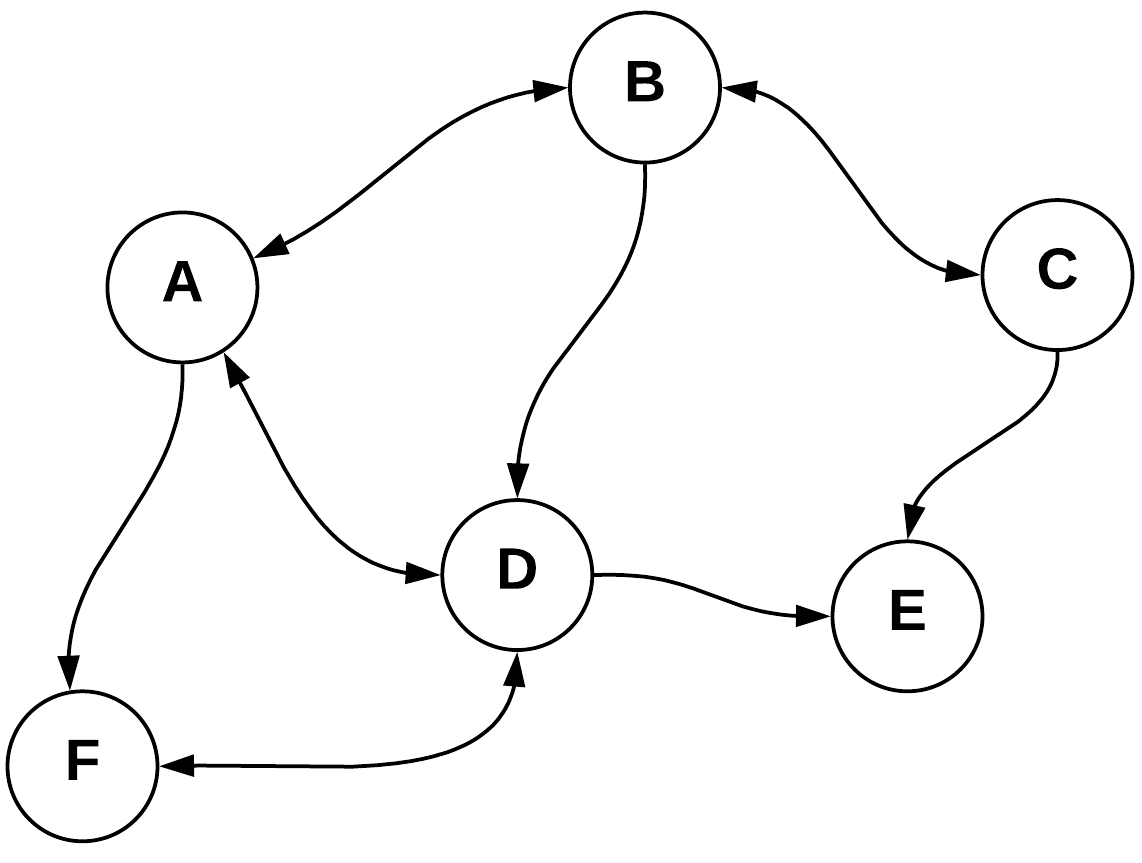
\includegraphics[width=0.5\columnwidth]{sections/figs/graph.png}
    % \end{center}
    % The above graph can be thought as a representation of different places in a city (represented by the nodes), and the lines with the arrows represent the roads connecting these different places. A line with two arrows allow two-way traffic, while line with single arrow only allow one way traffic. The connectivity between the different places can be summarized though the connectivity matrix $\mf{C} \in \mb{R}^{n \times n}$, where $n$ is the number of nodes in the graph. The elements of this connectivity matrix  represents whether or not there is a direct path between two places.
    % \[ 
    % c_{ij} = \begin{cases}
    %     1 & \text{there is a direct road between places } i \, \& \,j. \\
    %     0 & \text{otherwise.}
    % \end{cases}
    % \]
    % The diagonal element of $\mf{C}$ are zero, $c_{ii} = 0$.

    % Write down the connectivity matrix $\mf{C}$ for the graph shown above. How can we use the matrix $\mf{C}$ to answer the following questions? Explain exact matrix operation you would perform to answer these questions (Hint: Consider higher power of $\mf{C}$).
    % \begin{enumerate}
    %     \item Is there a path between two places $i$ and $j$ that goes via one other place? For example, we can go from $A$ to $D$ via $B$.
    %     \item How many paths are there between places $i$ and $j$ that goes via three other places?
    % \end{enumerate}
\end{enumerate}
% \newpage

% -*- root: ../assignment.tex -*-
\chapter{Orthogonality}

\begin{enumerate}[resume]
    \item Consider an orthonormal set of vectors,
    $$V = \left\{ \mf{v}_1, \mf{v}_2, \ldots \mf{v}_r\right\},\,\,\, \mf{v}_i \in \mb{R}^n\,\,\,\forall i \in \left\{1, 2, \ldots r\right\}$$
    If there is a vector $\mf{w} \in \mb{R}^n$ such that $\mf{v}_i^T\mf{w} = 0\,\,\,\forall i \in \left\{1, 2, \ldots r\right\}$. Prove that $\mf{w} \notin span\left(V\right)$.
    
    \item Consider the following set of vectors in $\mb{R}^4$.
    \[ V = \left\{
    \bmx
    1\\-2\\0\\3
    \emx,
    \bmx
    1\\1\\1\\1
    \emx,
    \bmx
    2\\-1\\1\\4
    \emx
    \right\} \]
    Find the set of all vectors that are orthogonal to $V$?

    \item For a matrix $\mf{A} \in \mb{R}^{m \times n}$, prove that $C\lp\mf{A}\rp \perp N\lp\mf{A}^T\rp$ and $C\lp\mf{A}^T\rp \perp N\lp\mf{A}\rp$.

    \item If the columns of a matrix $\mf{A} \in \mb{R}^{n \times n}$ are orthonormal, prove that $\mf{A}^{-1} = \mf{A}^T$. What is $\mf{A}^T\mf{A}$ when $\mf{A}$ is rectangular $\left(\mf{A} \in \mb{R}^{m \times n}\right)$ with orthonormal columns?

    \item What will happen when the Gram-Schmidt procedure is applied to: (a) orthonormal set of vectors; and (b) orthogonal set of vectors? If the set of vectors are columns of a matrix $\mf{A}$, then what are the corresponding $\mf{Q}$ and $\mf{R}$ matrices for the orthonormal and orthogonal cases?

    \item Consider the linear map, $\mf{y} = \mf{Ax}$, such that $\mf{x}, \mf{y} \in \mb{R}^n$ and $\mf{A} \in \mb{R}^{n \times n}$. Let us assume that $\mf{A}$ is full rank. What conditions must $\mf{A}$ satisfy for the following statements to be true,
    \begin{enumerate}
        \item $\Vert \mf{y} \Vert_2 = \Vert \mf{x} \Vert_2$, for all $\mf{x}, \mf{y}$ such that $\mf{y} = \mf{Ax}$.
        \item $\mf{y}_1^T\mf{y}_2 = \mf{x}_1^T\mf{x}_2$, for all $\mf{x}_1, \mf{x}_2, \mf{y}_1, \mf{y}_2$ such that $\mf{y}_1 = \mf{A}\mf{x}_1$ and $\mf{y}_2 = \mf{A}\mf{x}_2$. 
    \end{enumerate}
    \vspace{-0.1cm}
    \begin{color}{black!60}\small{\textbf{Note}: A linear map $\mf{A}$ with the aforementioned properties preserves lengths and angle between vectors. Such maps are encountered in rigid body mechanics.}
    \end{color}

    \item Prove that the rank of an orthogonal projection matrix $\mf{P}_{S} = \mf{UU}^T$ onto a subspace $\mc{S}$ is equal to the $\text{dim } \mc{S}$, where the columns of $\mf{U}$ form an orthonormal basis of $\mc{S}$.

    \item If the columns of $\mf{A} \in \mb{R}^{m \times n}$ represent a basis for the subspace $\mc{S} \subset \mb{R}^m$. Find the orthogonal projection matrix $\mf{P}_\mc{S}$ onto the subspace $\mc{S}$.
    
    {\color{gray} Hint: Gram-Schmidt orthogonalization.}

    \item Consider two orthogornal matrices $\mf{Q}_1$ and $\mf{Q}_2$. Is the $\mf{Q}_2^T\mf{Q}_1$ an orthogonal matrix? If yes, prove that it is so, else provide a counter-example showing $\mf{Q}_2^T\mf{Q}_1$ is not orthogonal.

    \item Let $\mf{P}_\mc{S}$ represent an orthogonal projection matrix onto to the subspace $\mc{S} \subset \mb{R}^n$. How can we obtain an orthonormal basis for $\mc{S}$ from $\mf{P}_\mc{S}$.

    \item Consider a 1 dimensional subspace spanned by the vector $\mf{u} \in \mb{R}^n$. What kind of a geometric operation does the matrix $\mf{R} = \mf{I} - 2\frac{\mf{u}\mf{u}^T}{\mf{u}^T\mf{u}}$ represent?
    
    Show that $\mf{R}$ satisfies the following properties:
    \begin{enumerate}
        \item $\mf{R}^2 = \mf{I}$
        \item Consider a vector $\mf{x} = \bmx x_1 & x_2 & \cdots & x_n \emx^\top \in \mb{R}^n$ such that $x_1 \neq 0$. If we choose $\mf{u} = $
    \end{enumerate}

    \item Prove that when a triangular matrix is orthogonal, it is diagonal.

    \item If an orthogonal matrix $\mf{Q} \in \mb{R}^{n \times n}$ is to be partitioned such that, $\mf{Q} = \bmx \mf{Q}_1 & \mf{Q}_2\emx$, then prove that $C\lp\mf{Q}_1\rp \perp C\lp\mf{Q}_2\rp$.

    \item Find an orthonormal basis for the subspace spanned by the following set,
    $$\lc \bmx1\\-1\\2\emx, \bmx-1\\-1\\-1\emx, \bmx1\\-3\\3\emx \rc$$

\end{enumerate}

\newpage

\end{document}